\documentclass{vgtc}                          % final (conference style)
%\documentclass[review]{vgtc}                 % review
%\documentclass[widereview]{vgtc}             % wide-spaced review
%\documentclass[preprint]{vgtc}               % preprint
%\documentclass[electronic]{vgtc}             % electronic version

\graphicspath{{figs/}}
\usepackage{times}
\renewcommand*\ttdefault{txtt}
\usepackage{mathptmx}
\usepackage{amsmath}

% Define \etal command
\newcommand{\etal}{\textit{et al.}}

% comment in following line for Japanese text
% \usepackage[whole]{bxcjkjatype}

\onlineid{0}
\vgtccategory{Research}
\vgtcinsertpkg
%\preprinttext{To appear in an IEEE VGTC sponsored conference.}
%\ieeedoi{xx.xxxx/TVCG.201x.xxxxxxx}

%% Paper title.

\title{StoryGem-NC: A Non Convex Region Extension for Meaning Preserving Voronoi Treemap Text Visualizations}

%% This is how authors are specified in the conference style

%% Author and Affiliation (single author).
%%\author{Roy G. Biv\thanks{e-mail: roy.g.biv@aol.com}}
%%\affiliation{\scriptsize Allied Widgets Research}

%% Author and Affiliation (multiple authors with single affiliations).
%%\author{Roy G. Biv\thanks{e-mail: roy.g.biv@aol.com} %
%%\and Ed Grimley\thanks{e-mail:ed.grimley@aol.com} %
%%\and Martha Stewart\thanks{e-mail:martha.stewart@marthastewart.com}}
%%\affiliation{\scriptsize Martha Stewart Enterprises \\ Microsoft Research}

%% Author and Affiliation (multiple authors with multiple affiliations)
\author{Naoya Oda \thanks{e-mail: oden6680@gmail.com}\\ \scriptsize Nihon University %
\and Yosuke Onoue \thanks{e-mail: onoue.yousuke@nihon-u.ac.jp}\\ \scriptsize Nihon University}

% \teaser{
%   \centering
%   \includegraphics[width=17cm]{teaser.pdf}
%   \caption{teaser image}
% }

\teaser{
  \centering
  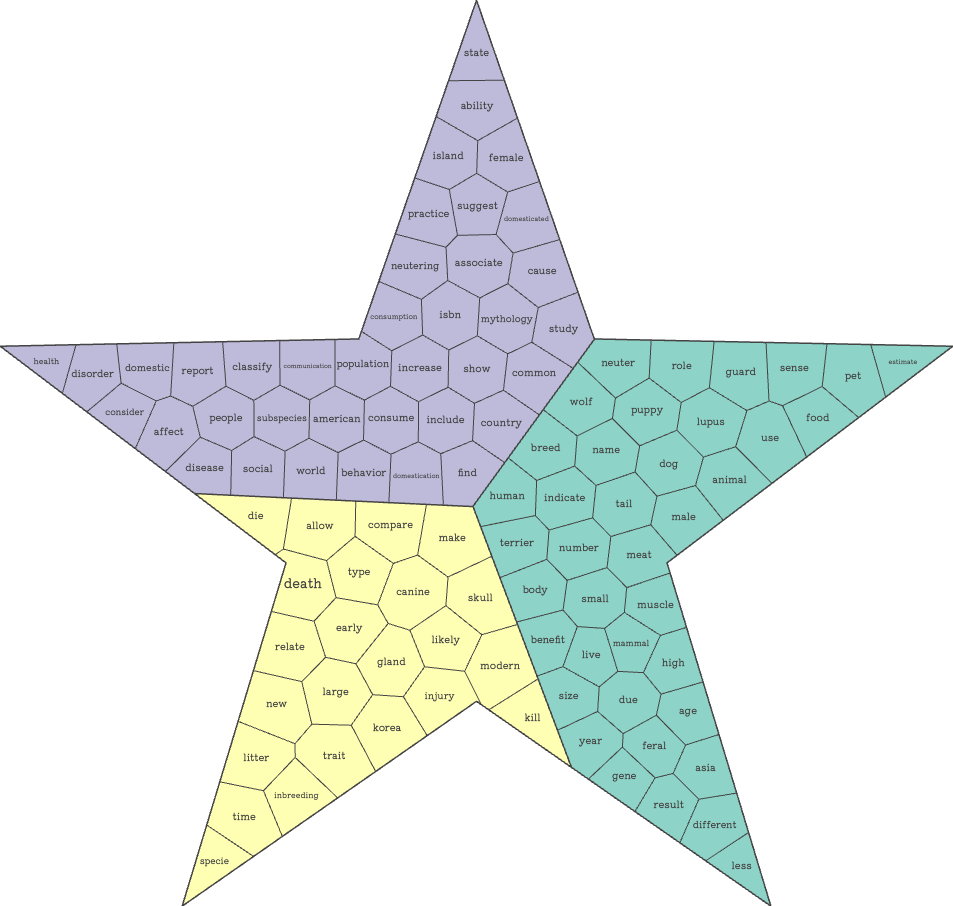
\includegraphics[width=0.45\textwidth]{figs/star.png}
  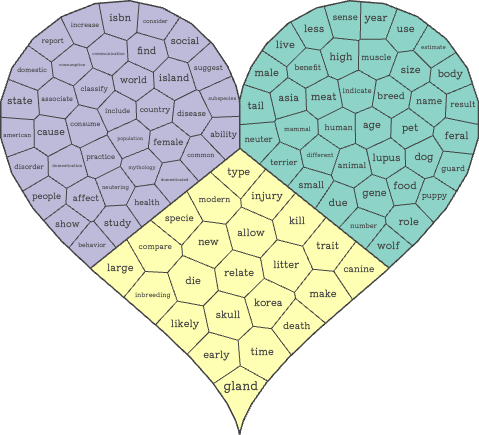
\includegraphics[width=0.45\textwidth]{figs/heart.png}
  \caption{
    Examples of StoryGem-NC applied to non convex shapes using text from Wikipedia's Dog article: (a) star shaped region and (b) heart shaped region. The method successfully fills these complex shapes while maintaining semantic relationships between dog related terms.
  }
  \label{fig:teaser}
}

\abstract{
  StoryGem is a text visualization technique that addresses WordCloud's inability to capture semantic connections and SemanticWordCloud's difficulty in efficiently filling defined areas.
  However, StoryGem is limited to convex regions.
  We present StoryGem-NC (non convex), an extension that enables execution on non convex regions.
  While processing non convex regions incurs higher computational costs, our experiments confirm practical performance for web based applications.
  This extension opens new possibilities for visualizations using geographical boundaries, corporate logos, and other meaningful shapes.
}

\CCScatlist{
  \CCScatTwelve{Human-centered computing}{Visualization}{Visualization application domains}{Information visualization}
  \CCScatTwelve{Human-centered computing}{Visualization}{Visualization techniques}{Treemaps}
}

% \nocopyrightspace

%%%%%%%%%%%%%%%%%%%%%%%%%%%%%%%%%%%%%%%%%%%%%%%%%%%%%%%%%%%%%%%%
%%%%%%%%%%%%%%%%%%%%%% START OF THE PAPER %%%%%%%%%%%%%%%%%%%%%%
%%%%%%%%%%%%%%%%%%%%%%%%%%%%%%%%%%%%%%%%%%%%%%%%%%%%%%%%%%%%%%%%%

\begin{document}
\firstsection{Introduction}
\maketitle

WordCloud is a ubiquitous text visualization method that arranges words with varying sizes to represent importance.
However, traditional WordClouds use random layouts that fail to convey semantic relationships between words, limiting their analytical value for understanding text structure and meaning.

SemanticWordCloud and similar approaches attempt to preserve word relationships through spatial proximity but struggle with efficiently packing words into fixed areas.
This challenge becomes even more complex when dealing with non rectangular display regions.
ShapeWordle~\cite{8807355} demonstrated the value of filling arbitrary shapes with words, showing that non convex region support has practical merit for creating visually engaging and contextually appropriate visualizations.

StoryGem~\cite{oda2025storygemvoronoitreemapapproach} introduced a novel approach using Voronoi treemaps to create continuous layouts where area encodes importance, avoiding the overemphasis of long words while preserving semantic relationships.
User studies confirmed that this approach helps viewers better understand text structure and identify related concepts.
However, StoryGem's reliance on the \texttt{d3-voronoi-treemap} library restricts it to convex polygonal display regions, limiting its applicability to real world visualization scenarios.

In this paper, we present StoryGem-NC, an extension supporting arbitrary non convex domains while maintaining practical performance for web based applications.
This advancement enables new visualization possibilities for geographic data, branded content, and educational materials.

\section{Method}

StoryGem-NC extends the original StoryGem framework to support non convex regions through three main stages with critical modifications.

\paragraph{Building a Semantic Word Network}
The preprocessing pipeline removes stop words and uses NLTK part of speech tagging to retain only verbs, nouns, and adjectives.
Word embeddings are extracted using a pretrained FastText model (157 languages, trained on CommonCrawl and Wikipedia), ensuring broad language coverage and semantic quality.
A $k$-nearest neighbor graph is constructed by computing cosine similarity between word pairs, creating a network that reflects semantic structure.
This network forms the foundation for subsequent clustering and layout operations.

\paragraph{Hierarchical Clustering and Voronoi Treemap Layout}
The Louvain method detects communities in the word network, creating reproducible hierarchical clusters that group semantically related terms.
These clusters are arranged using Balzer \etal's~\cite{balzer2005voronoi} Voronoi treemap algorithm, which performs iterative centroidal Voronoi tessellation.
This process allocates cell areas proportional to word weights (typically term frequency), creating a gapless layout that can fill non convex regions while maintaining area based importance encoding.
The key innovation is that this algorithm naturally handles non convex boundaries without modification.

\paragraph{Font Size Adjustment for non convex Cells}
The original StoryGem's font size optimization assumes convex cells, which fails for non convex regions where cells themselves may become non convex.
Our solution adopts a more general approach: we use a uniform base font size of 10 pixels and compute each text's bounding box radius $r_0$ from its dimensions.
For each cell, we calculate the minimum distance $r$ from the cell's centroid to any of its edges, ensuring text remains within boundaries.
The scaling factor is determined as:
\[
  s = \min\left(\frac{r}{r_0}, 1\right)
\]
This ensures text fits within available space regardless of cell convexity.


\section{Application Examples}

To demonstrate the effectiveness of our non convex extension, we applied StoryGem-NC to text data from Wikipedia's Dog article, visualizing it within star and heart shapes (Figure~\ref{fig:teaser}).
These shapes were specifically chosen to test the method's ability to handle both sharp concave angles and smooth curves, representing the diverse geometries encountered in practical applications.

The star shaped visualization (Figure~\ref{fig:teaser}a) presents particular challenges due to its five sharp inward pointing vertices.
Despite these geometric constraints, our method successfully preserves the semantic clustering of dog related terms.
This robustness to extreme concavity is crucial for applications requiring complex shapes.

The heart shaped visualization (Figure~\ref{fig:teaser}b) tests our method's handling of smooth, curved boundaries combined with a sharp inward cusp at the top.
The algorithm adapts gracefully to these varying geometric properties, filling the space completely while maintaining semantic coherence.
The smooth distribution of words across the curved boundaries demonstrates the method's versatility.

These examples reveal several key strengths of StoryGem-NC:
\begin{itemize}
  \item \textbf{Shape Flexibility}: The method successfully adapts to arbitrary non convex shapes without manual intervention or shape specific parameters
  \item \textbf{Semantic Preservation}: Hierarchical clustering and spatial proximity of semantically related words remain intact despite geometric constraints
  \item \textbf{Practical Performance}: Both visualizations were generated in 5-10 seconds for datasets containing 50-100 words
  \item \textbf{Visual Quality}: Words are legibly sized and positioned, avoiding overlaps while maximizing space utilization
\end{itemize}

The successful handling of these non convex shapes suggests numerous practical applications beyond decorative visualizations.
Geographic boundaries could visualize region specific text data, corporate logos could display company terminology, and educational materials could use meaningful shapes to enhance learning and retention.

\section{Conclusions}

We have presented StoryGem-NC, a significant extension of the StoryGem text visualization technique that removes the constraint of convex only display regions.
By adapting the font size adjustment algorithm and leveraging the inherent flexibility of Voronoi treemaps, we enabled meaningful text visualizations within arbitrary non convex shapes while preserving the semantic relationships that make StoryGem valuable.

Our experiments with star and heart shapes demonstrate that the method successfully handles both sharp concave angles and smooth curves, maintaining semantic clustering even under challenging geometric constraints.
The practical performance of 5-10 seconds for typical datasets (50-100 words) confirms that StoryGem-NC is suitable for interactive web applications, opening new possibilities for contextually appropriate visualizations.

The ability to use non convex shapes has significant implications for practical applications.
Geographic boundaries can now be used to visualize region specific text data, with words filling the actual shape of countries, states, or districts.
Corporate logos can display company related terminology, creating branded visualizations that reinforce visual identity.
Educational materials can leverage meaningful shapes—such as a brain for neuroscience terms or a leaf for botanical vocabulary—to create memorable, context appropriate visualizations.

However, several challenges remain for future work.
First, the current font size adjustment strategy, while functional for non convex cells, lacks the optimization elegance of the original convex only approach.
Developing more sophisticated optimization techniques for non convex cells represents an important research direction.
Second, the current implementation requires predefined polygon shapes; a more flexible system would allow users to import arbitrary shapes from image files and handle complex topologies including regions with holes.
Finally, while our performance is acceptable for moderate sized datasets, scaling to larger corpora may require algorithmic optimizations or GPU acceleration.

Despite these limitations, StoryGem-NC represents a meaningful step toward more flexible and expressive text visualizations.
By enabling semantic word layouts within non convex shapes, we provide designers and analysts with new tools for creating visualizations that are both informative and visually aligned with their content's context.

\bibliographystyle{abbrv-doi}
\bibliography{reference}
\end{document}
